%%%%%%%%%%%%%%%%%%%%%%%%%%%%%%%%%%%%%%%%%
%%% WP01
%%%%%%%%%%%%%%%%%%%%%%%%%%%%%%%%%%%%%%%%%

\tsubsubsection{WP03 - Access to RI for Accelerators}

%%%%%%%%%%%%%%%%%%%%%%%%%%%%%%%%%%%%%%%%%
%%% Section content, please change!
%%%%%%%%%%%%%%%%%%%%%%%%%%%%%%%%%%%%%%%%%

\subsubsection*{Overview and Goals}

\begin{table}[H]
    \renewcommand{\arraystretch}{1.50}		
    \footnotesize   
    \begin{tabular}{*{3}{|p{0.10\textwidth}}|l|}
        \hline
        \rowcolor{mygray} \multicolumn{4}{|c|}{\textit{\color{white}Work Package Summary}} \\
        \hline
        \rowcolor{mylightergray} \textit{WP No.} & \cellcolor{white} 01 & \textit{Title of WP} & \cellcolor{white} WP Title \\
        \hline
        \rowcolor{mylightergray} \textit{Start} & \cellcolor{white} Mxx & \textit{End} & \cellcolor{white} Myy \\
        \hline
        \rowcolor{mylightergray} \multicolumn{4}{|p{0.978\textwidth}|}{\textit{Participating Organisations}} \\
        \hline
        \multicolumn{4}{|p{0.978\textwidth}|}{
            \hspace*{-0.75cm} 
            \begin{minipage}[t]{\textwidth}
    			\begin{itemize}
    			    \item WP Leader: Partner 1
    				\item Participants: Partner 2, Partner 3, Partner 4, Partner 5, Partner 6, Partner 7
    			\end{itemize} 
    			\vspace*{0.10em}
			\end{minipage}
        } \\
        \hline
    \end{tabular}
    \vspace{0.5em}\vfill
    \begin{tabular}{|p{0.978\textwidth}|}
        \hline
        \rowcolor{mylightergray} \textit{Goals} \\
        \hline
        \rowcolor{white} 
        \hspace*{-0.75cm} 
        \begin{minipage}[t]{\textwidth}
    		\begin{itemize}
    		    \item Goal 1
    			\item Goal 2
			    \item Goal 3
    		\end{itemize} 
    		\vspace*{0.10em}
		\end{minipage}        
        \\
        \hline
    \end{tabular}
    \vspace{0.5em}\vfill
    \begin{tabular}{|l|*{7}{>{\centering\arraybackslash}p{0.084\textwidth}|}}
        \hline    
        \rowcolor{mylightergray} \textit{Participant number} & \textit{1} & \textit{2} & \textit{3} & \textit{4} & \textit{5} & \textit{6} & \textit{7} \\
        \hline
        \rowcolor{white} \cellcolor{mylightergray}\textit{Participant short name} & Partner 1 & Partner 2 & Partner 3 & Partner 4 & Partner 5 & Partner 6 & Partner 7 \\
        \hline
        \rowcolor{white} \cellcolor{mylightergray}\textit{PM per participant} & xx & xx & xx & xx & xx & xx & xx \\
        \hline        
    \end{tabular}    
\end{table}

\subsubsection*{Status}

\todo{Briefly explain the status of the WP.}

\subsubsection*{Progress per Task}

\subparagraph{Task no: 3.1 Material Testing Facilities} \mbox{}

This task includes the High-Radiation to Materials (HiRadMat) Faclity at CERN. 

HiRadmat has had great progress in the last reference period concerning EURO-LABS. The facility remains in extremely high demand from the international community, involving both EU and overseas teams that are performing experiments. A total of 3928 AUs have been spend (from the total requested 4800). The percentage of AUs spent vs the available AUs are shown in Figure~\ref{fig:stat_pie_hiradmat}. Given the high demand for the facility also in view of the CERN's long shutdown between 2026-2029, HiRadMat could welcome also more access units in case they become available, in order to support the experiments in 2026. 

\begin{figure}[!h]
    \centering
    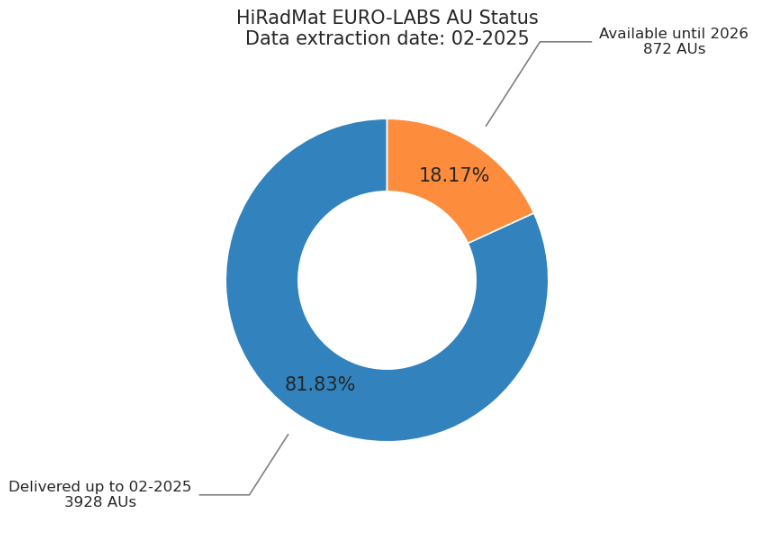
\includegraphics[width=0.75\linewidth]{graphics/stat_pie_hiradmat.png}
    \caption{Access Units spent in HiRadMat in all reference periods. A total of 4800 AUs were allocated in total ; 3696 AUs have been already spent in this second reference period, and 232 AUs have been spent after September 2024 and until today (Feb. 2025). }
    \label{fig:stat_pie_hiradmat}
\end{figure}

For the funded users, the gender distribution is shown also in Figure~\ref{fig:gender_distr_hiradmat}, removing the duplicates by name. 

\begin{figure}[!h]
    \centering
    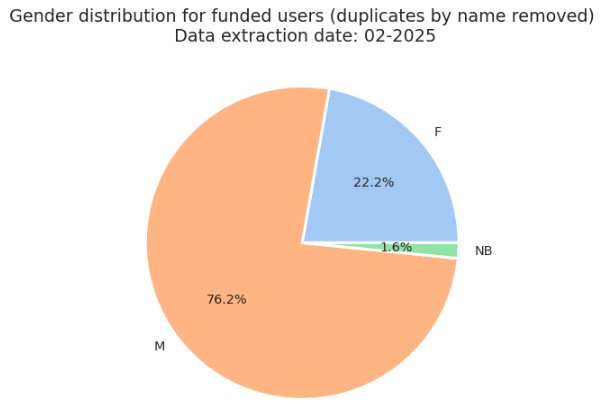
\includegraphics[width=0.6\linewidth]{graphics/gender_distr_hiradmat.png}
    \caption{Gender distribution of TA funded users for Task Force 3.1 (HiRadMat)}
    \label{fig:gender_distr_hiradmat}
\end{figure}

The age distribution of the funded users, is indicating that as per the instructions for TA, the user selection panel has approved mostly undergraduate and postgraduate students, at the early stages of their careers and fewer senior researchers (professors and tenured researchers). However, specifically at HiRadMat, the presence of the senior persons in the preparatory, data-taking and experimental phases is absolutely necessary for the success of the experiments. The age distribution for the funded users is shown in Figure~\ref{fig:age_distr_hiradmat}.

\begin{figure}[!h]
    \centering
    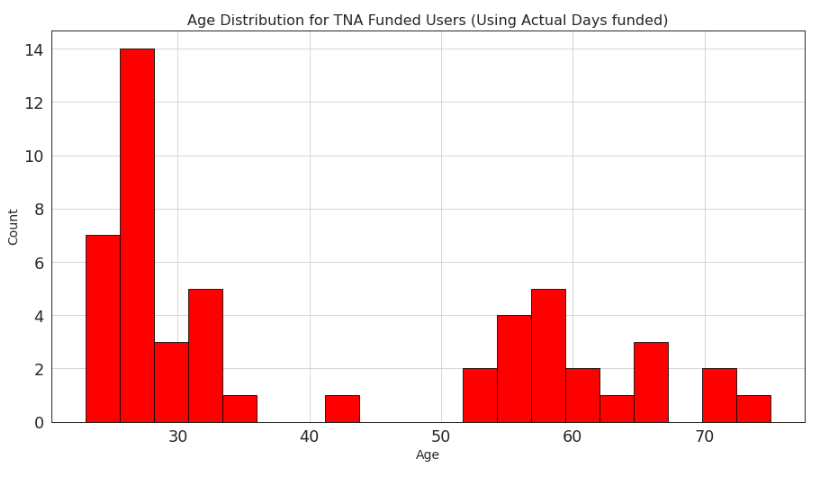
\includegraphics[width=0.75\linewidth]{graphics/age_distr_hiradmat.png}
    \caption{Age distribution of funded users in Task 3.1 (HiRadMat). The majority of the supported users is at the early stages of their career, while a few senior researchers or recognized scientists at their field have been also necessary during the preparatory or the post-irradiation phases.}
    \label{fig:age_distr_hiradmat}
\end{figure}

The evolution of the spent access units overall, and only for the RP2 is shown in Figures~\ref{fig:overall_evolution_hiradmat} and~\ref{fig:RP2_evolution_hiradmat}.

\begin{figure}[!h]
    \centering
    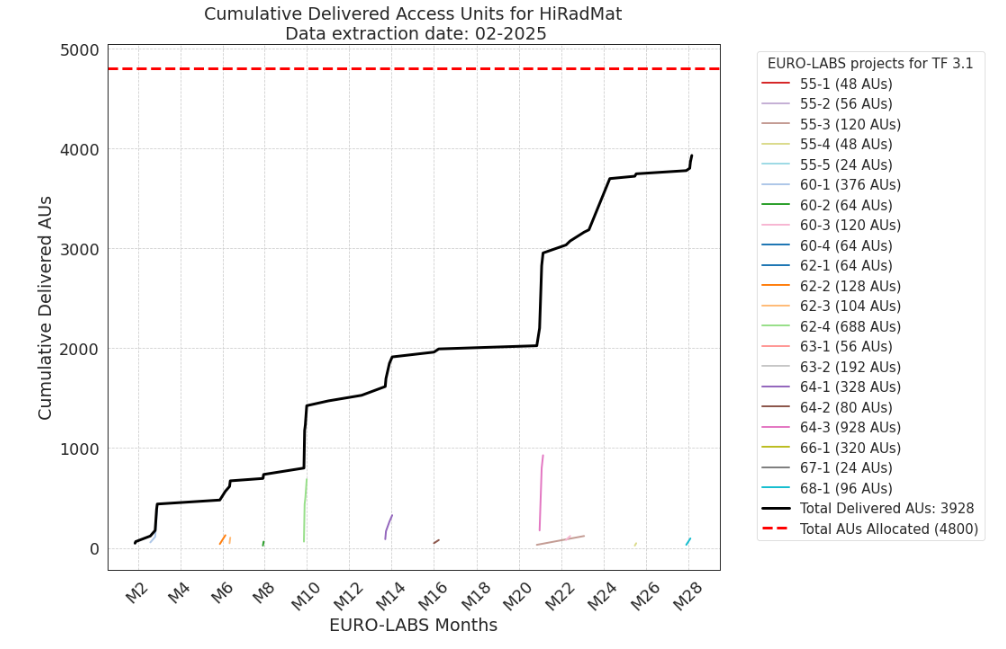
\includegraphics[width=0.9\linewidth]{graphics/overall_evolution_hiradmat.png}
    \caption{Overall evolution of delivered AUs for HiRadMat and breakdown of AUs per project.}
    \label{fig:overall_evolution_hiradmat}
\end{figure}

\begin{figure}[!h]
    \centering
    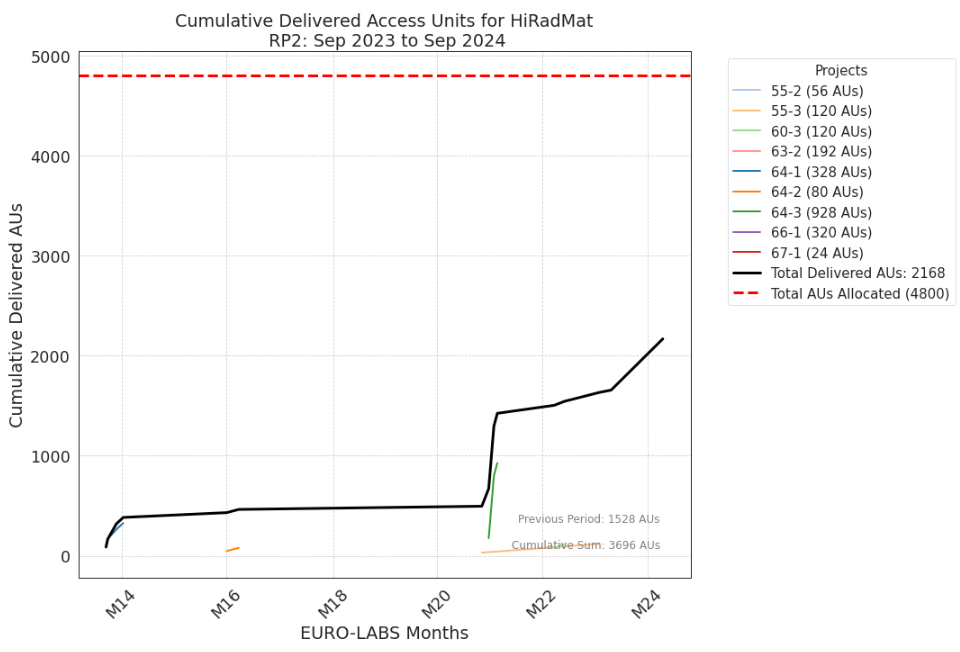
\includegraphics[width=0.9\linewidth]{graphics/RP2_evolution_hiradmat.png}
    \caption{Evolution of delivered AUs for HiRadMat during the second reference period (RP2) and breakdown of AUs per project.}
    \label{fig:RP2_evolution_hiradmat}
\end{figure}

\subsubsection*{Main Results and Achievements}

Many of the HiRadMat experiments produced great results during this second reference period. The results of the \textbf{HRMT-62} and \textbf{HRMT-64} experiments have an extremely high impact. In particular, up to-date, 5 peer-reviewed articles have been written, 3 of them published in or submitted to Nature, all citing the EURO-LAB support. In total, 14 press releases have been done by the collaborating institutes, including 2 from CERN (bulletin \& courrier). It worth noting that the articles have a high ``attention score'', of 260: 99th percentile of the 329,972 tracked articles of a similar age in all journals. The key scientific result from HRMT-64, only made possible with the EURO-LABS support, was the first-time measurement of the magnetic fields produced by plasma instabilities using a Faraday rotation, seen in Figure~\ref{fig:hiradmat_mag_field_plasma}.

\begin{figure}[!h]
    \centering
    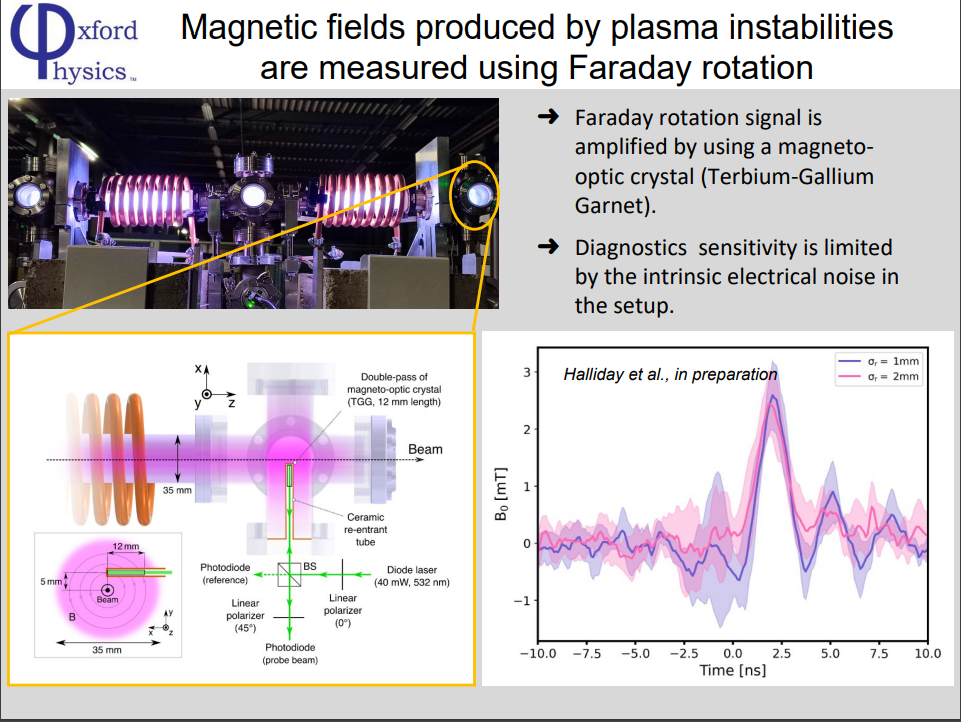
\includegraphics[width=0.75\linewidth]{graphics/HRMT_64_magnetic_field.png}
    \caption{HRMT-64, with the EURO-LABS support measured for first time the magnetic fields produced by plasma instabilities using a faraday rotation in HiRadMat. Courtesy: Prof. G. Gregori, Univ. of Oxford.}
    \label{fig:hiradmat_mag_field_plasma}
\end{figure}

\textbf{HRMT-66} was a novel experiment that pushed forward our current knowledge of material limits, particularly for the often used Glassy Carbon and Beryllium, along with a first-time irradiation of Si$_{3}$N$_{4}$ in order to investigate its exact damage threshold. This is very important for the cooling section of a future muon collider. A photo from the results is shown in Figure~\ref{fig:hiradmat_Si3N4} for Si$_{3}$N$_{4}$ and in Figure~\ref{fig:hiradmat_GC} for Glassy Carbon. 

\begin{figure}[!h]
    \centering
    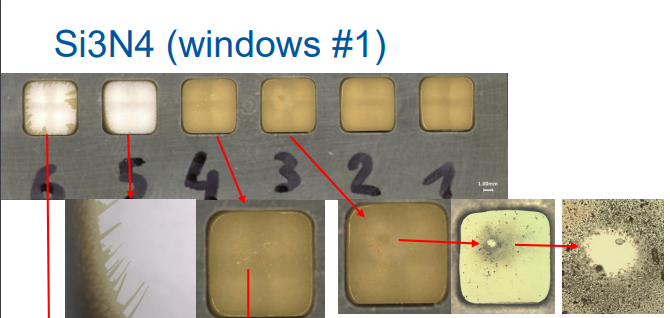
\includegraphics[width=0.75\linewidth]{graphics/hiradmat_si3n4.png}
    \caption{Beam impact on Si3N4 windows during HRMT-66 experiment. The support of EURO-LABS was extremely important since FLUKA simulations were absolutely necessary for the evaluation of the damage mechanisms and precence at CERN was vital for some of the collaborators of the experiment.(Courtesy: A. Harrison, CERN)}
    \label{fig:hiradmat_Si3N4}
\end{figure}

\begin{figure}[!h]
    \centering
    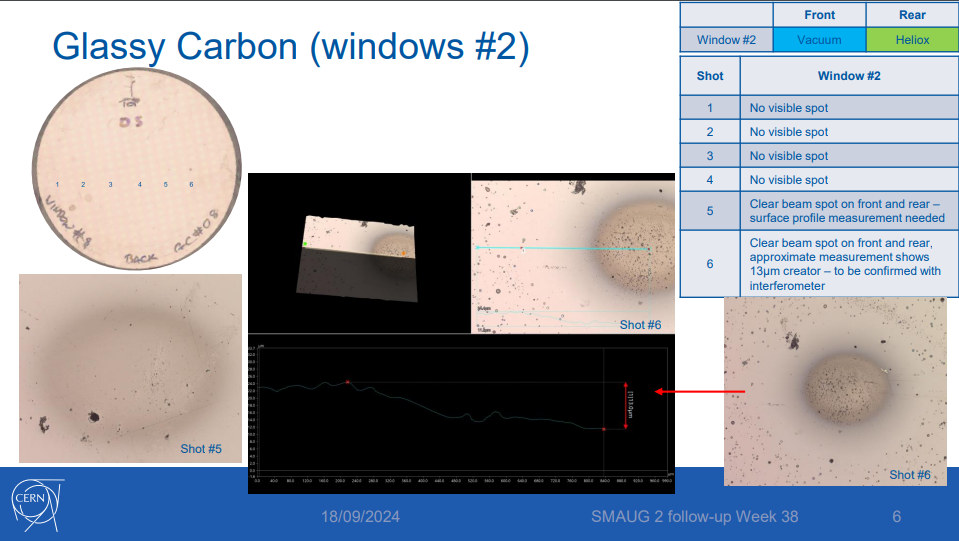
\includegraphics[width=0.75\linewidth]{graphics/hiradmat_GC.png}
    \caption{Results from HRMT-66 experiment on Glassy Carbon. The clearb beam spot can be seen in shot \#6 including a small crater.}
    \label{fig:hiradmat_GC}
\end{figure}

\textbf{HRMT-55} concluded in 2024, and a follow-up experiment, \textbf{HRMT-71}
is planned to take place in 2025. This is a collaboration between CERN and ESS, with the results being useful for both organisations.

The results indicate similar detector performance for all ionisation chambers (IC), however detector to detector performance differences were observed. See for example Figure~\ref{fig:hiradmat_IC_response}. In order to complete documentation and validate future designs, \textbf{HRMT-71} will also request funding from EURO-LABS, in particular for the ESS relevant part. 

\begin{figure}[!h]
    \centering
    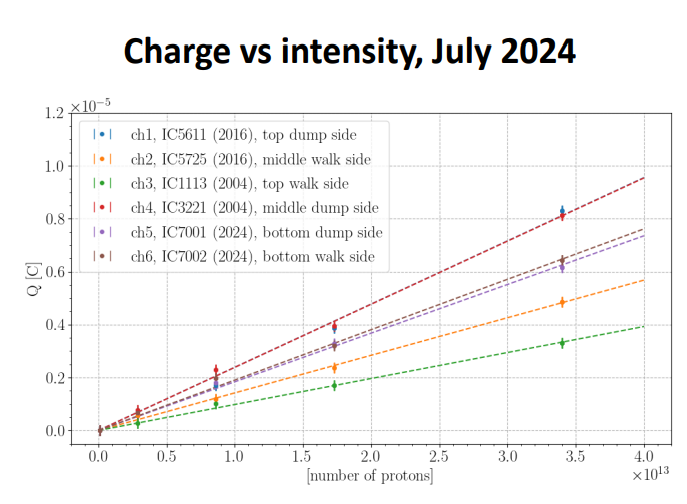
\includegraphics[width=0.8\linewidth]{graphics/hiradmat_IC_response.png}
    \caption{Response (C) of the different ionization chambers tested in HRMT-55. The difference in the slope needs to be understood in detail in a follow-up experiment (HRMT-71) planned for 2025. (Courtesy. S. Grishin, ESS)}
    \label{fig:hiradmat_IC_response}
\end{figure}

\subsubsection*{Progress in the service improvements tasks assigned for HiRadMat}

EURO-LABS is supporting a service improvement part for HiRadMat that is focused on improving the calibration of the SPS Beam Position Monitor System (designated ``ALPS'), that also affects HiRadMat. The beam position precision, in particular for experiments like HRMT-62 and HRMT-64 is very important, and for the moment is not fully reliable. 

As part of this task, a neural network is being developed that would improve the residual errors for the device calibration, that today is done via a simple polynomial fit. 

The task is quite complicated and with ambiguous results : The performance of the existing calibration curve was never studied in this way before. This task is well ongoing (via a doctoral student that works at CERN in collaboration with Univ. of Oxford). 

It needs to be noted that the algorithm of choice will be developed by the end of 2025 and a report will be written by then. However \textbf{no implementation can happen before 2029}, i.e after the CERN long shutdown. This aligns with the timeline and the schedule for this particular task of the project, since it will allow proper prototyping and testing of the new electronic components during the CERN long shutdown between 2026-2029. 

First preliminary results comparing the residuals produced by a neural network vs the old polynomial fit approach, taking into account the response of a single electrode of an ALPS Beam Position Monitor (BPM), can be seen in Figure~\ref{fig:hiradmat_SI}. Further optimization studies towards the minimization of errors in terms of beam position measurements are ongoing.
\begin{figure}[!h]
    \centering
    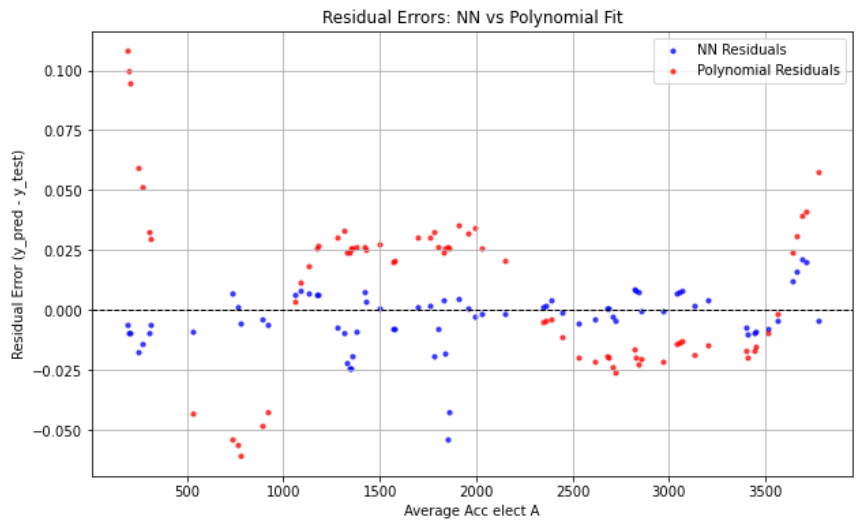
\includegraphics[width=0.75\linewidth]{graphics/hiradmat_SI.png}
    \caption{Residuals for the calibration curve of an ALPS beam position monitor, for the response of a single electrode. The newly developed neural network seems to outperform the old polynomial fit. (Courtesy, V. Stergiou, A. Boccardi (CERN)).}
    \label{fig:hiradmat_SI}
\end{figure}

\subsubsection*{Deviations and Corrective Actions}

HiRadMat has spent in the second reference period already 82\% of the 4800 allocated AUs. This is due to the facility's publicity (also thanks to EURO-LABS dissemination efforts and the promotional videos). The AUs left can cover a part of the 2025 experiments, however there will be no budget left to support the rest of the 2025 and the 2026 experiments (the number of which is, currently uncertain). Therefore, in case that other facilities will not manage to spend, HiRadMat would welcome some additional funding for TA and for support to the users with logistics and simulations. 

\subsubsection*{Milestones and Deliverables}

{\fontsize{9}{11}\selectfont
\begin{center}
  \begin{tabular}[t]{!{\color{mygray}\vrule}p{0.10\linewidth}!
  {\color{mygray}\vrule}p{0.60\linewidth}!
  {\color{mygray}\vrule}p{0.20\linewidth}!{\color{mygray}\vrule} } \hline
    \rowcolor{mycyan} & {\bf Title} & {\bf Status} \\ \hline
    \cellcolor{mycyan}{\bf D1.x}: &  &  \\ \hline
  \end{tabular}
\end{center}
}

\subparagraph{Task no 2 : Technology Infrastructures} \mbox{}

\todo{Briefly explain the progress of the task in context to the DoA.}

\subsubsection*{Main Results and Achievements}

\todo{Briefly summarise the main results and achievements of the WP in context of the DoA.}

\subsubsection*{Deviations and Corrective Actions}

\todo{Briefly summarise any deviations and performed corrective actions of the WP in context of the DoA.}

\subsubsection*{Milestones and Deliverables}

{\fontsize{9}{11}\selectfont
\begin{center}
  \begin{tabular}[t]{!{\color{mygray}\vrule}p{0.10\linewidth}!
  {\color{mygray}\vrule}p{0.60\linewidth}!
  {\color{mygray}\vrule}p{0.20\linewidth}!{\color{mygray}\vrule} } \hline
    \rowcolor{mycyan} & {\bf Title} & {\bf Status} \\ \hline
    \cellcolor{mycyan}{\bf D1.x}: &  &  \\ \hline
  \end{tabular}
\end{center}
}


\subparagraph{Task no 3 : Electron and Plasma Beams} \mbox{}

\todo{Briefly explain the progress of the task in context to the DoA.}

\subsubsection*{Main Results and Achievements}

\todo{Briefly summarise the main results and achievements of the WP in context of the DoA.}

\subsubsection*{Deviations and Corrective Actions}

\todo{Briefly summarise any deviations and performed corrective actions of the WP in context of the DoA.}

\subsubsection*{Milestones and Deliverables}

{\fontsize{9}{11}\selectfont
\begin{center}
  \begin{tabular}[t]{!{\color{mygray}\vrule}p{0.10\linewidth}!
  {\color{mygray}\vrule}p{0.60\linewidth}!
  {\color{mygray}\vrule}p{0.20\linewidth}!{\color{mygray}\vrule} } \hline
    \rowcolor{mycyan} & {\bf Title} & {\bf Status} \\ \hline
    \cellcolor{mycyan}{\bf D1.x}: &  &  \\ \hline
  \end{tabular}
\end{center}
}


\subparagraph{Task no 4 : Applications} \mbox{}

\todo{Briefly explain the progress of the task in context to the DoA.}
Task 3.4 includes two facilities: the INTC/RAPID and the CERN/CLEAR.

\subsubsection*{Main Results and Achievements}

\todo{Briefly summarise the main results and achievements of the WP in context of the DoA.}


In the reporting period 2 INCT Rapid infrastructure provided access with EURO-LABS support carrying out 7 projects (one projects is still ongoing). The experiments were carried using the following instruments: 
•	LAE 10 accelerator with nanosecond pulse radiolysis sat-up – to investigate basic mechanisms of ionising radiation interactions in biological systems.
•	Electronica accelerator, generating beam of electrons of energy 10 MeV – for sterilization and materials modification
•	ILU 6 accelerator, using electron beam of energy 1.7 MeV and energies < 300 keV – for controlled depth of electron range in treated products.
For the experiments carried out at RPAID infrastructure the dosimetry measurements were performed by INCT Labotartru of Technological Dose Measurements, to ensure precise and accurate dose delivery in treated samples. Also additional INCT infrastructure supported carried out experiments was used, e.g Electron Paramagnetic Spectroscopy to help characterise radiation induced effects in materials.
The experiments were focused on application of electron beam to investigate the mechanisms of radicals interactions, radiation induced effects in materials and effects of electron beam irradiation on food and food ingredients: 
•	One-electron oxidation of S-adenosyl methionine,
•	Crosslinking of self-assembled fatty acids on copper by electron beam irradiation,
•	Effect of ionizing irradiation on dried fruits,
•	Influence of 10 MeV accelerated electrons on structure and properties of sheep wool fibres as a potential component for preparation of polymer-based composite materials
•	Irradiation engineering of biopolymer-based formulation for wound management and targeted drug delivery devices,
•	Bioactivity of irradiated foods by low energy e-beam,
•	Face masks recycling with the use of radiation technologies.
In the upcoming year it is planned to adjust experimental set-up for irradiation in gaseous phase, as a response to newly received project request. This will broaden the area of research carried out at INCT within EURO-LABS.



\subsubsection*{Deviations and Corrective Actions}

\todo{Briefly summarise any deviations and performed corrective actions of the WP in context of the DoA.}

\subsubsection*{Milestones and Deliverables}

{\fontsize{9}{11}\selectfont
\begin{center}
  \begin{tabular}[t]{!{\color{mygray}\vrule}p{0.10\linewidth}!
  {\color{mygray}\vrule}p{0.60\linewidth}!
  {\color{mygray}\vrule}p{0.20\linewidth}!{\color{mygray}\vrule} } \hline
    \rowcolor{mycyan} & {\bf Title} & {\bf Status} \\ \hline
    \cellcolor{mycyan}{\bf D1.x}: &  &  \\ \hline
  \end{tabular}
\end{center}
}


\subsubsection*{Project Meetings}

%  {\color{mygray}\vrule}p{0.40\linewidth}!

%%%%%%%%%%%%%%%%%%%%%%%%%%%%%%%%%%%%%%%%%